\section{Семантика примитивов\\
пользовательского уровня\\
с точки зрения сборки мусора}

Одним из самых популярных алгоритмов сборки мусора является  алгоритм ``\emph{пометки и 
освобождения}'' (mark-and-sweep). Его популярность обусловлена простотой и тем, что 
данный алгоритм накладывает минимальные ограничения на организацию поддержки времени
исполнения и требует минимальной поддержки со стороны компилятора. 

Задачи, решаемые в процессе организации сборщика мусора такого типа, показаны на Рис.~1.

\begin{figure}[h!]
	\centering
	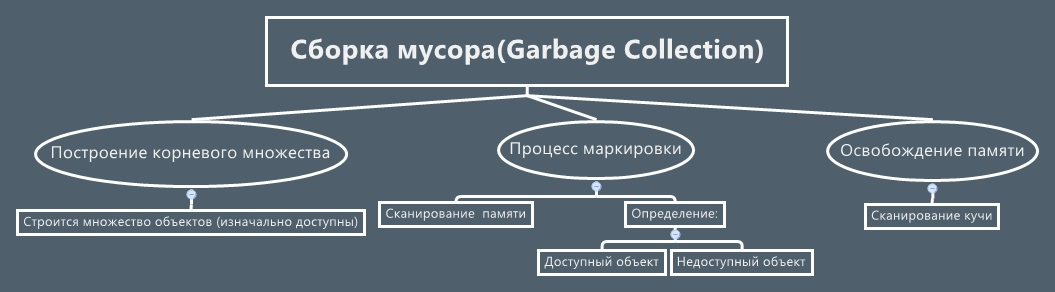
\includegraphics[width=500pt]{picture1.jpg}
	\caption{Три основных этапа сборки мусора}
	\centering
\end{figure}

Алгоритм ``пометки и освобождения'' состоит из двух фаз, которые запускаются последовательно
одна за другой:

\begin{itemize}
\item Фаза пометки. Начиная с некоторого аксиоматически заданного множества указателей, называемого
\emph{корневым множеством}, происходит полный обход всех достижимых объектов. Каждый достижимый
объект помечается как живой.
\item Фаза освобождения. Происходит полный обход кучи, во время которого освобождается память
из-подо всех непомеченных объектов; при этом пометка с помеченых объектов снимается.
\end{itemize}

Для реализации сборки мусора с помощью алгоритма ``пометки и освобождения'' должны быть решены
следующие задачи:

\begin{enumerate}
\item Идентификация корневого множества. Корневое множество~--- это множество указателей на
объекты, которые считаются изначально доступными для программы. Такие указатели хранятся в
стеке, регистрах и статической области памяти. В задачу идентификации корневого множества 
входит распознавание указателей в кучу на отведенные там объекты среди всех таких значений.

\item Определение всех ссылок из данного объекта на другие объекты в куче, что необходимо для
обхода всех достижимых объектов в фазе пометки.

\item Обеспечение возможности пометки объектов в куче и обхода всей кучи с освобождением 
непомеченных объектов.
\end{enumerate}

Последняя задача относится к реализации кучи; её решение изложено в~\cite{realisation}. Ниже 
мы опишем, как с помощью пользовательских примитивов, введенных в предыдущем разделе,
нами решаются две первые задачи.

\subsection{Поддержка корневого множества}

Идентификация корневого множества указателей (то есть указателей, хранящихся на стеке, в регистрах и статической
области памяти) без помощи со стороны компилятора является серьезной проблемой~\cite{roots}. При ``библиотечном''
подходе к сборке мусора рассчитывать на поддержку со стороны компилятора не приходится, поэтому в момент
начала сборки мусора идентифицировать корневые указатели уже невозможно. Поэтому корневое множество
поддерживается по мере работы программы. В него добавляются все \lstinline{gc_ptr}, экземпляры которых
не созданы с помощью \lstinline{gc_new}. Для этого в функции \lstinline{gc_new} выставляется флаг,
который проверяется в конструкторе \lstinline{gc_ptr}; в этом же конструкторе происходит добавление
указателя на объект \lstinline{gc_ptr} в пул корней, если это необходимо. Удаление же корневого
указателя происходит при вызове его деструктора. Так как удалять нужно только корневые указатели, а деструкторы
вызываются для всех, в \lstinline{gc_ptr} хранится признак того, что это корень. Поскольку деструкторы 
вызывается по отношению к конструкторам в обратном порядке (для автоматических объектов), пул корней можно 
реализовать в виде стека в отдельной области памяти вне кучи. 

\subsection{Построение метаинформации}

Представление метаинформации для сборки мусора, использованное нами, близко к тому, что описано
в~\cite{meta}. Метаинформация для типа представляет собой вектор смещений объектов \lstinline{gc_ptr} 
относительно начала экземпляра этого типа. Функция \lstinline{gc_new}, используемая для создания объектов, 
осуществляет поиск метаинформации по имени типа, полученному с помощью функции \lstinline{typeid}. 
Если этот поиск неуспешен (и, следовательно, для данного типа еще не была построена метаинформация), 
то создается новый объект, хранящий метаинформацию, и ассоциируется с именем этого типа. Для построения
метаинформации используются вызовы конструкторов \lstinline{gc_ptr}, с помощью которых можно
посчитать разность между адресом начала объекта и адресом, по которому ``внутри'' него расположен данный
\lstinline{gc_ptr}. 

После получения метаинформации функция \lstinline{gc_new} размещает указатель на неё перед данными 
создаваемого объекта. Это даёт возможность по указателю на живой объект узнать все указатели
из него на другие живые объекты, то есть реализовать стадию маркировки.
